%TODO Hodai: get rid of the CPU (use processor/computational time...)
%TODO Gera: Covariance -> Variance
%TODO Hodai: find the correct word for "guarded automata"

\documentclass[11pt]{article}

\usepackage{graphicx}
\usepackage{tikz}
\usetikzlibrary{shapes.geometric, arrows, automata, positioning}
\tikzstyle{recNode} = [rectangle, minimum width=3cm, minimum height=1cm, text centered, rounded corners=0.1cm, draw=black]
\tikzstyle{recNodeB} = [recNode, draw=blue, fill=blue!10,text=blue!20!black]
\tikzstyle{recNodeG} = [recNode, draw=red, fill=red!10,text=red!10!black]
\tikzstyle{eNode} = [minimum height=1cm, text centered,text=blue!20!black]

\tikzstyle{arrow} = [thick,->,>=stealth,draw=black]
\tikzstyle{arrowB} = [thick,->,>=stealth,draw=blue]
\tikzstyle{arrowG} = [ultra thick,->,>=stealth,draw=red, dashed]

%\usepackage{float}
%\usepackage{etoolbox}
%\usepackage{cite}
\usepackage{url}
%\patchcmd{\thebibliography}{\section*}{\section}{}{}

\author{Hodai Goldman (Hodaig@cs.bgu.ac.il) \\ \\Department of Computer Science, \\Ben-Gurion University of the Negev, Beer Sheva, Israel \\ \\Supervisor: Dr. Gera Weiss}
\date{\today}
\title{Research Proposal: Computational resource management of multi channel controller}

\begin{document}
\begin{titlepage}
\maketitle
\end{titlepage}



\section{Background and Problem Statement}
\label{sec:Background}
Today's computer power allows for consolidation of controllers allowing systems where a single computer regulates many control loops, each with its varying needs of computation resources.
This brings two research challenges that we intend to attack in the proposed thesis:
\begin{itemize}
	\item How to schedule control tasks in order to achieve good performance in terms of control measures (overshoot, convergence speed, etc.)?
	\item What is a good interface for co-design of scheduling and control?
\end{itemize}

While it is possible to build control systems using standard operating systems, either real-time or desktop, with static or with dynamic scheduling schemes, there is an agreed opinion in the control community that these do not serve well for the purpose outlined above \cite{??}. Specifically, desktop type operating systems (Windows, Linux, etc.) schedule for computational efficiency but do not allow for worst-case performance guarantees of the individual tasks that regulate the loops. On the other hand, real-time operating systems sacrifice some efficiency for timing predictability but the type of timing guarantees that such systems provide are not enough to be used for guaranteeing control performance. When using such operating systems for control engineers usually apply controllers that work in a fixed periodic manner so that control behavior becomes deterministic and control performance can be guaranteed. This is not efficient because resources can be better utilized if controllers act at higher frequencies when only when needed. 
In this work we will develop methods to combine the efficiency of desktop operating systems with the predictability of real-time operating systems in a way that is more suitable for control systems then periods and deadlines

The control loops that we are analyzing have the architecture shown in Figure~\ref{fig:control loop}. 
We assume a close feedback control loop where the physical plant, \textit{System}, is monitored via an array of sensors (\textit{Sensing}) which produce raw data that represents some state variables. 
We assume uncertainty observations from the sensors so after sensing the \textit{State Estimator} aggregates the raw data from all the sensors and makes an educated estimation of the current state in order to improve the state estimation. Then the \textit{Control Law} will use actuators (change the outputs)  in order to close the gap from the current estimated state and the reference state (\textit{Input}).

The current state of the art is that control engineers design control tasks as periodic computations then they specify the required periodic frequency for the task and software engineers design a scheduler that ensures that the periodic frequency requirements are met usually using pre-computed knowledge of the expected (maximum) duration of the tasks.
We claim that for control systems we can achieve better performance by using richer and more flexible set of requirements for the tasks. Specifically, we will develop tools with which the control engineers can specify in a natural way features of their control loop that the scheduler will use to allow for dynamic schedules that guarantee required control performance. 

\begin{figure}[]
    \centering
    
    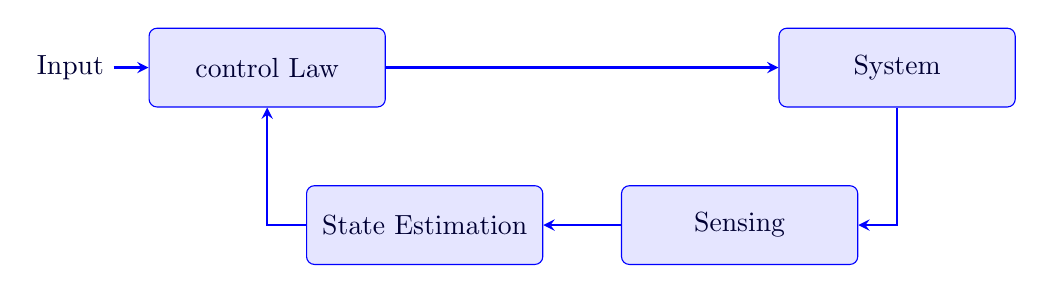
\begin{tikzpicture}[node distance=2cm]
        \node (in) [eNode] {Input};
        \node (control) [recNodeB, right of=in, xshift=0.5cm] {control Law};
        \node (sys) [recNodeB, right of=control, xshift=6cm] {System};
        \node (sensor) [recNodeB, below of=sys, xshift=-2cm] {Sensing};
        \node (estimator) [recNodeB, below of=control, xshift=2cm] {State Estimation};
        
        \draw [arrowB] (in) -- (control);
        \draw [arrowB] (control) -- (sys);
        \draw [arrowB] (sys) |- (sensor);
        \draw [arrowB] (sensor) -- (estimator);
        \draw [arrowB] (estimator) -| (control);
    \end{tikzpicture}
    
    \caption{A typical control loop system.
    \label{fig:control loop}}
\end{figure}


%In this thesis we suggest a novel technique where the control loop is composed (as usual) from control tasks and state estimation tasks. 
%And the requirement of the periodical requirements of the control tasks dynamically change and depend on the level of the environmental noise that is expressed by the accuracy of the state estimation (retrieve from estimation loops) and the stability of the system (retrieve from the control loop).


\section{Case studies}
\label{sec:Case study}

\subsection{Vision based controllers for drones}
To test our concepts, we will examine the implementation of an autonomously flying quad-rotor in the context of an agriculture case study. Specifically, we will implement a quad-rotor that flies in corridors and greenhouses by a vision based feedback. The challenge in this case study, from our perspective, is that image processing is a heavy computational task that requires careful scheduling in order to preserve the system predictability and stability.

The current state-of-the-art solution for involving heavy computational tasks such as vision in the control system is simply by adding computational power to the system (use faster processors), usually much more than needed in order to eliminate the chance of loosing predictability.
Some, more conservative, control engineers prefers to isolate the heavy computation from the core control loop by allocating one of the processor's core for that task, or even run the vision processing on a different computer (see, for example, how APM suggest to use computer vision abilities~\cite{APM}).

In Section~\ref{sec:Research Plan} we suggest a novel framework model for such systems that we will implement in this thesis.

\subsection{Nano-Satellite}
Another interesting case study we will examine is the control of a nano-satellite, in particular scheduling the sensing tasks of \textit{IAI}\footnote{IAI: Israel Aerospace Industries} nano satellites. Their satellites are controlled by a small and relatively slow processor, and the developers say that the main issue in programing the satellite is how to schedule the sensing tasks.
The common approach they are using is to periodically schedule all the sensing task every iteration, and they say that this is the main computational consumption and is too much for their slow processor.

We think that lots of the sensing are unnecessary and the controlling task can be achieved without "most up-to-date" information, some times we can base on good estimation of the sensing value or even use the last value. Although Vision based drones is our main case study, we will also check the possibility to improve the nano-satellite issue with our framework.

\section{Research Plan}
\label{sec:Research Plan}

Our research plan consists of: (1) Designing a methodology for effective allocation of computational resources in real-time control systems; and then (2) Demonstrating our methodology with a framework for developing such systems and with a case study. The details of these two steps are elaborated below.


\begin{figure}[]
    \centering
    
    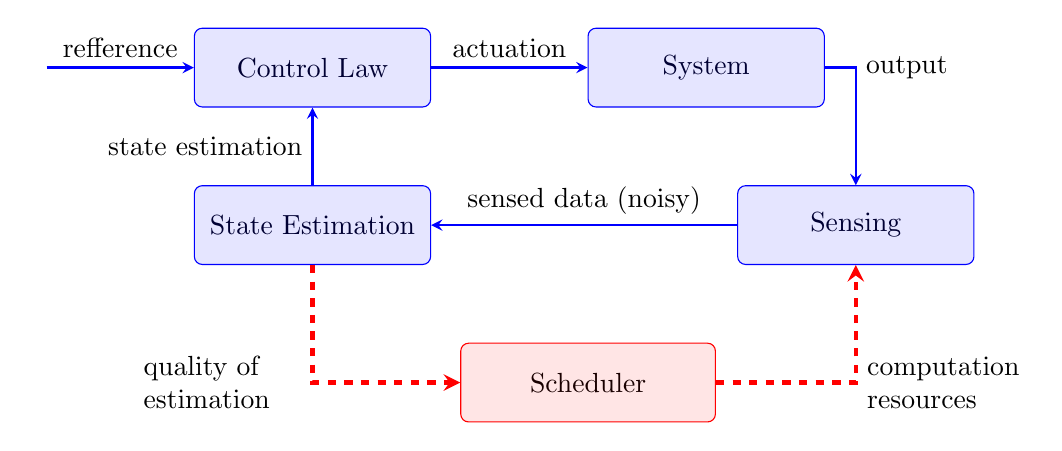
\begin{tikzpicture}[node distance=2cm]
        \node (in) [eNode] {};
        \node (control) [recNodeB, right of=in, xshift=1.5cm] {Control Law};
        \node (sys) [recNodeB, right of=control, xshift=3cm] {System};
        \node (sensor) [recNodeB, below of=sys, xshift=1.9cm] {Sensing};
        \node (estimator) [recNodeB, below of=control] {State Estimation};
        \node (sched) [recNodeG, below of=estimator, xshift=3.5cm, text width=3cm] {Scheduler};
        
        \draw [arrowB] (in) -- node[above] {refference} (control);
        \draw [arrowB] (control) -- node[above] {actuation} (sys);
        \draw [arrowB] (sys) -| node[right] {output} (sensor);
        \draw [arrowB] (sensor) -- node[above] {sensed data (noisy)} (estimator);
        \draw [arrowB] (estimator) -- node[left] {state estimation} (control);
        
        \draw [arrowG] (sched) -| node[right,text width=2cm] {computation resources} (sensor);
        %\draw [arrowG] (sched) --  node[right] {$cov(v)$} (estimator);
        \draw [arrowG] (estimator) |- node[left,text width=2cm] {quality of estimation} (sched);
        
        
    \end{tikzpicture}
    
    \caption{Our proposal of a general controller framework. Each control loop (depicted in blue) informs the resource allocator (Scheduler) of its quality of estimation and the allocator allocates accordingly the computation resources among all the control loops. The noise in the sensed data is a function of the amount of computation resources. The more resources are invested in sensing the better (less noisy) sensed data is obtained.
    \label{fig:general_hybrid_loop}}
\end{figure}

\begin{figure}[h]
    \centering
    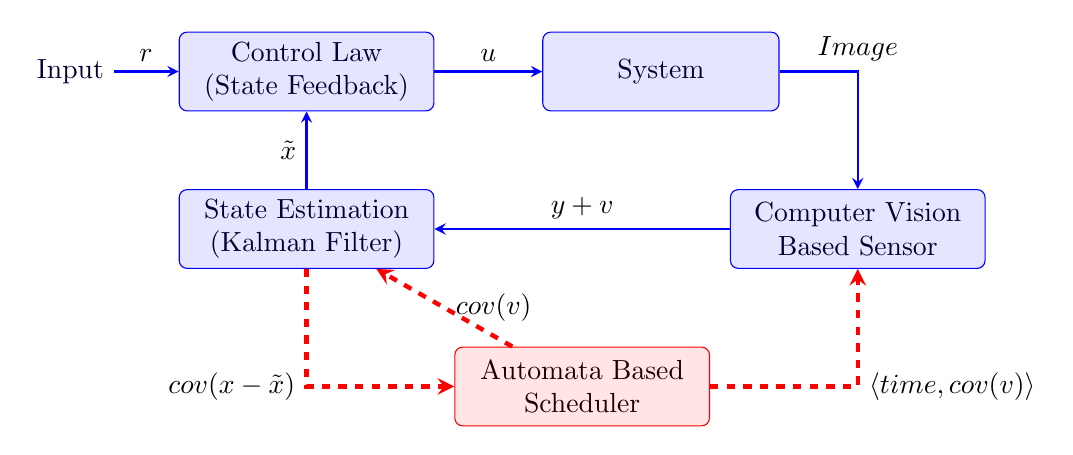
\begin{tikzpicture}[node distance=2cm]
        \node (in) [eNode] {Input};
        \node (control) [recNodeB, right of=in, xshift=1cm, text width=3cm] 
            {Control Law (State Feedback)};
        \node (sys) [recNodeB, right of=control, xshift=2.5cm] {System};
        \node (sensor) [recNodeB, below of=sys, xshift=2.5cm, text width=3cm] 
            {Computer Vision Based Sensor};
        \node (estimator) [recNodeB, below of=control, text width=3cm] 
            {State Estimation (Kalman Filter)};
        \node (sched) [recNodeG, below of=estimator, xshift=3.5cm, text width=3cm] {Automata Based Scheduler};
        
        \draw [arrowB] (in) -- node[above] {$r$} (control);
        \draw [arrowB] (control) -- node[above] {$u$} (sys);
        \draw [arrowB] (sys) -| node[above] {$Image$} (sensor);
        \draw [arrowB] (sensor) -- node[above] {$y+v$} (estimator);
        \draw [arrowB] (estimator) -- node[left] {$\tilde{x}$} (control);
        
        \draw [arrowG] (sched) -| node[right] {$\langle time,cov(v) \rangle$} (sensor);
        \draw [arrowG] (sched) --  node[right] {$cov(v)$} (estimator);
        \draw [arrowG] (estimator) |- node[left] {$cov(x-\tilde{x})$} (sched);
        
    \end{tikzpicture}
    
    \caption{The controller framework we will implement, the \textit{scheduler} will allocate CPU time ($\langle time,cov(v) \rangle$) for the \textit{Computer Vision} task base on the state estimation certainty using guarded Automata.
    \label{fig:hybrid_loop}}
\end{figure}

\subsection{The proposed methodology}
\label{sec:our proposal}

The general methodology that we will develop is illustrated in Figure~\ref{fig:general_hybrid_loop}.
The methodology comes to support an efficient scheduling protocols in modern control systems consisting of a computer that runs many tasks that implement the control laws of independent control loops. 
The current state of art is that the designers of each control loop specify a fixed rate for invocations of the corresponding control task.
%That methodology is based on modern controller architecture where the system has multiple controlling tasks (control loops) and a scheduler that schedule the task as they demand.
% TODO: Use the terminology of the figure
In our methodology, shown in Figure~\ref{fig:general_hybrid_loop}, there is a strong relation between the \textit{Scheduler} and the control loops. We suggest that each control loop (blue components) will tell the resource allocator (\textit{scheduler}) its level of certainty and the allocator will allocate the CPU time among all the control loops corresponding to the loops certainty in order to maintain some pre-defined specifications of state certainty or stability.

Our proposal is general and may be applicable in a wide range of applications. However, in this initial phase of the research, we believe that it is better to focus on a specific sub-domain and solve all technical issues in order to prove the concept.
In this thesis we will develop and implement the framework shown in Figure~\ref{fig:hybrid_loop}: a vision based controller for drone. 

As shown in Figure~\ref{fig:hybrid_loop}, the suggested control system framework have strong relation between the tasks scheduler to the control loops, in this case the estimation task (\textit{State~Estimation}) accuracy strongly depends on the sensing task (\textit{Computer~Vision}) and there both collaborate with the \textit{scheduler} in order to achieve they \textbf{control objectives} (g.e. stability).
In this framework the scheduler is part of the control logic and therefore it can make scheduling decisions based on the current control state, the scheduling of \textit{Computer~Vision} task is depends on the accuracy of state estimation.
For example if the vision is clear the \textit{Computer~Vision} will produce good measurement of the \textit{System} and therefore good accuracy will be achieved so the \textit{Scheduler} can allocate less computation time to the heavy \textit{Computer~Vision} task and still remain stable and allocate more CPU to others control loops or some background tasks (like navigation).

The above collaboration requires to re-adjust some parts of the controlling system, e.g. the \textit{State~Estimator} needs to work with variable error covariance of \textit{Computer~Vision} measurement and the \textit{Computer~Vision} needs to be able run within variable time limits, and also the tasks pre-defined requirements need to be re-adjust in order to define the relation between tasks, like \textit{Computer~Vision} and \textit{State~Estimator}.
Below we will dive in each part of the above system (Figure~\ref{fig:hybrid_loop}) and explain how it will be adjusted (changed) and how we will achieve that adjustment in our demonstration.

%Finally, we need to re-consider the system Analyzing technique because variable sensing characteristics (\textit{Computer~Vision} time limits) will lead to variable estimation characteristics... %TODO - complete and fix this paragraph or remove it

\subsubsection{Sensors (\textit{Computer~Vision~Based~Sensor})}
\label{sec:sensors}
%Anitime reserch of zilbershtain (\cite{Shlomo})
%contract based
%http://ardupilot.org/copter/docs/common-mouse-based-optical-flow-sensor-adns3080.html

\textit{Computer~Vision~Based~Sensor} is the module that is responsible for taking picture or series of pictures and for producing measurements of quantities such as speed and position relative to the environment.
In our research we will use the \textit{Computer~Vision} in order to detect two dimensional movement in the camera surface (i.e. the drone speed).
There are many such algorithms (optical flow), they differ by their running time and by the accuracy of the solution, mostly more time lead to more accuracy.

In our case we need to be able to control the \textit{Computer~Vision} running time and to have some good knowledge of the solution accuracy in order to achieve optimal state estimation (see Section~\ref{sec:estimator}).
We assume that the \textit{Computer~Vision} error is spread normally, and we will use the error covariance as the solution accuracy. 
We believe that this is a reasonable  assumption because it is the sum of many independent random variables, as follows. Optic flow algorithms usually go by identifying similar regions in consecutive pictures and then averaging the distances that each feature ``traveled''. Assuming that the error in measurement of each feature is independent of the other errors, we get that the total error is the average of independent random variables. We will validate this assumption by experimentation with different parameters of different algorithms.

%TODO - reed a litle the article (\cite{UPenn-Pant}) and re-write the next.
%TODO - check if Anitime reserch (\cite{Shlomo}) can fit here.
%TODO - Make sure that we use the terms contract-base and any-time correctly
In order to control the running time, we will use anytime based algorithms~\cite{Shlomo} and will mainly concentrate on ``contract based" vision algorithms proposed by Pant~\cite{UPenn-Pant}.
This type of algorithms run until we stop them, and when we stop them they will provide a solution with accuracy that is proportional to the amount of time it was running. That way we can control the solution accuracy by controlling the running time.
In our implementation, in order to lower the complexity, we will pre-define few different ``operation modes" of the \textit{Computer~Vision} task, that differ by their running time and they are identified by a pair $\langle RunTime, Covariance \rangle$ where $Covariance$ is the error covariance of running time $RunTime$.

\subsubsection{State Estimator}
\label{sec:estimator}
% kalman filter & ...
% seperation rule of kalman

In cases where we have uncertain observations (inaccurate sensors), e.g. the computer vision measurement, we prefer to make some \textbf{educated estimation} of the current state based on the uncertain observations rather than just consider the last observation as the current state.
This \textbf{educated estimation} about the current state is the main goal of the \textit{State~Estimator} block.
This block receives the raw data from the sensors and produce an estimation of the current state.

In this thesis we will use well known optimal estimator called Kalman filter, or, more accurately, extended Kalman filter (EKF) which is the nonlinear version of Kalman filter.
The algorithm works in a two-step process. In the prediction step, the Kalman filter produces estimates of the current state variables, along with their uncertainties. Once the outcome of the next measurement is observed, these estimates are updated using a weighted average, with more weight being given to estimates with higher certainty.
%The algorithm is recursive. It can run in real time, using only the present input measurements and the previously calculated state and its uncertainty matrix; no additional past information is required. 
\cite{Kalman-filter}

In order to produce optimal estimation with Kalman filter, one of the parameter that we need to consider in our calculation is the variance of the sensor error.
But in our new framework the sensor (vision based sensor) have variable error variance for each time slot, this means that we need to have also variable state estimators correspondingly.
In order to adjust the sensor error variance, each time step the scheduler will inform the state estimator about the new error variance, and the state estimator will use corresponding parameters to make the next estimation.

APM, the control software that we will use, is already using kalman filter as the state estimator, so we only need to adjust the existing module to the variable sensor error variance, and to send the estimation error variance to the scheduler (see Section~\ref{sec:scheduler}).

\subsubsection{Control Tasks} 
\label{sec:control}
The control task itself (\textit{Control Law} in Figure~\ref{fig:general_hybrid_loop}) is responsible for reducing the difference between the current state ($x$) where $\tilde{x} = x+ ``estimation~error"$ (in Figure~\ref{fig:general_hybrid_loop}) and the target state ($u$ in Figure~\ref{fig:general_hybrid_loop}), by changing the drone motors speed.

%Optimal estimation or optimal control low is not guarantee the overall  optimal feedback controller, but as Kalman prove, 
The control task is usually a very low CPU consumer and been well studied~\cite{???}, hence, in this thesis we will not be concentrated on the control task, we will use the same controller that APM are using.
APM use a common used and well known technique from control theory called {\textbf{PID}\footnote{PID controller - A proportional-integral-derivative controller}}.
In this technique the control output is based on the physical knowledge of the system dynamics, and have 3 variable parameters (P, I and D) that define the controller convergence behavior.

We will also try to use ``adjustable'' {\textbf{LQR}\footnote{LQR - Linear-quadratic regulator}}.
LQR is an optimal controller that take into account the level of certainty of the state estimation. 
Is Usually hard task to know the certainty of estimation, but in our case we need to calculate it anyway, and we mark it as $cov(x-\tilde{x})$.
We will make LQR ``adjustable'' in the sense that each iteration the controller will consider the new (variable) $cov(x-\tilde{x})$.
We will check if adjustable LQR has significant advantages over PID in cases were we have variable certainty of estimation.

\subsubsection{Computation Resource Scheduler: Automata Based Scheduler}
\label{sec:scheduler}

Real-time systems are mostly composed of multiple real-time tasks, tasks with time constraint, for example task that must response within specified time constraints.
The purpose of schedulers in such systems is to allocate the limited computational resources (CPU time) within all the task in the system. To do so, we need a well defined communication interface between the real-time tasks and the scheduler.

The most common way of describing the requirements of a real-time component is to specify a period, sometimes along with a deadline, which gives the frequency at which the component must execute. The designer of the component makes sure that the performance objectives are met as long as the component is executed consistent with its period. The scheduler guarantees that all components get enough resources.
%not directly in this article
Specifying resource requirements using periods has advantages due to simplicity and analyzability, but has limited expressiveness \cite{RTComposer}. 
%For example, a specification such as “execute the component every 5ms” does not say whether the scheduler should or should not execute it more frequently if enough computing resources are available, and if a component has multiple methods, say, for different control tasks, each needing a different period, the requirement cannot be naturally captured by a single period.

In this thesis one of the main subjects, as we said above (Section~\ref{sec:Research Plan}), is to develop a methodology for allocation resources. We will focus on how should engineers describe the requirements of a real-time component.
To simplify, We will assume that the resource is allocated in discrete slots of some fixed duration in the style of time-triggered architecture~\cite{RTComposer}.
We will develop automata based (hybrid automata) methodologies and schedulers based on the work of Alur~\cite{RTComposer} and Bukra~\cite{Merav}, and will demonstrate with measurable data how they improve the performance of real flying drones (see Section~\ref{sec:results}).
%We will use finite automata over infinite words as specification framework for resource requirements, automata can be more expressive, for describe more specific requirements, and they are composable, it is easy to compose all the tasks requirements into one automata. 

We will use hybrid automata as specification framework for resource requirements.
hybrid automata is a variation of finite automata for infinite words~\cite{hibrid-systems}.
Automata can be more expressive for describe more specific requirements, and they are composable, it is easy to compose all the tasks requirements into one general automata.
The hybrid automata define continuous (fixed period) operation modes, represented by the automata state, and the condition of mode changing (mode transition) denote by the automata edges.
The operation mode directly define a set of tasks that will be executed in the time slot (for example $s_{0.7}$ in Figure~\ref{fig:sched_sense_auto}).
We can stay at a single mode for few time iterations, in this case the same tasks will be schedule in each iteration. 
We can also take \textbf{discrete mode transition} in order to change operation mode after few iterations and schedule different set of tasks, for example, in Figure~\ref{fig:sched_sense_auto} the edge $(m_1,m_2)$ says that if the previous iteration mode was $m_1$ and $estCov < 0.7$ we can change the mode and schedule the set $\{s_{0.2}\}$ in the next iteration.

Each infinite path on the composed hybrid automata (not necessary infinite mode transitions) is a scheduling that satisfy all the tasks requirements. 
In this architecture the scheduler only need to ``walk through'' the composed automata, this is of course fast and easy computational task. 
In order to assure that we not exceed the time slot duration, each task will have pre-defined maximum duration time like ``deadline'' in the traditional architecture. Now we can verify that every possible scheduling step can execute within a single time slot, in other words, every mode of the composed automata can be done in single time slot, by simply summarize the ``deadline'' of all the tasks in the mode tasks set.
%we can summarize the total slot ``deadline'' as follows:\\
%$\forall mode~e ~~(\sum_{t \in Guard(e)} deadline(t) ) \leq slot~duration$ \\
If we find mode that goes beyond the maximum duration we will remove it from the automata so we never exceed the time slot duration.


\begin{figure}[]
    \centering
    
    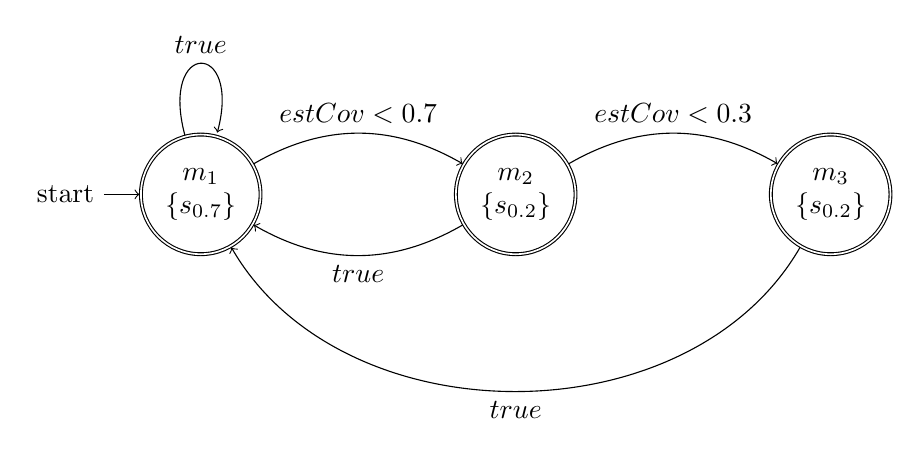
\begin{tikzpicture}[node distance=4cm, text centered, auto]
        \node (A) [state, accepting, text width=1cm, initial] {$m_1$ $\{s_{0.7}\}$};
        \node (B) [state, accepting, text width=1cm] [right of=A] {$m_2$ $\{s_{0.2}\}$};
        \node (C) [state, accepting, text width=1cm] [right of=B] {$m_3$ $\{s_{0.2}\}$};
        
        \path[->] (A) edge [loop above] node {$true$} (A);
        %\path[->] (A) edge [bend left] node {$\neg est_{bad} \wedge s_{0.2}$} (B);
        \path[->] (A) edge [bend left] node {$estCov < 0.7$} (B);
        \path[->] (B) edge [bend left] node {$true$} (A);
        %\path[->] (B) edge [loop above] node {$\neg cov3$} (B);
        %\path[->] (B) edge [bend left] node {$est_{good} \wedge s_{0.2}$} (C);
        \path[->] (B) edge [bend left] node {$ estCov < 0.3$} (C);
        %\path[->] (C) edge [loop above] node {$cov1$} (C);
        \path[->] (C) edge [bend left=60] node {$true$} (A);
                

    \end{tikzpicture}
    
    \caption{Example of guarded automata for our vision based sensor task, in this example the task has two operation modes, $\mathbf{s_{0.7}}$ which need 70\% of the time slot but is more accurate vision computation and $\mathbf{s_{0.2}}$ which is less accurate but faster (need only 20\% of the slot).
    The value of $estCov$ is $cov(x-\tilde{x})$ of the previous iteration.
    Every time slot exactly one of the modes will be executed.
    \label{fig:sched_sense_auto}}
\end{figure}

\begin{figure}[]
    \centering
    
    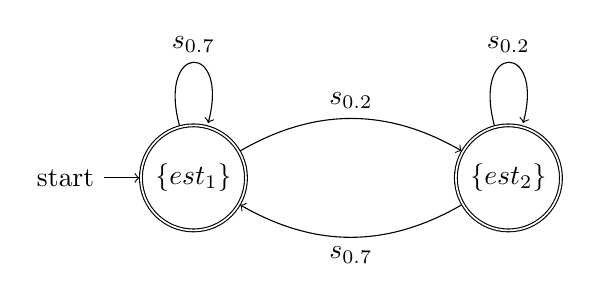
\begin{tikzpicture}[node distance=4cm,auto]
        \node (A) [state, accepting, initial] {$\{est_1\}$};
        \node (B) [state, accepting] [right of=A] {$\{est_2\}$};
        
        \path[->] (A) edge [loop above] node {$s_{0.7}$} (A);
        \path[->] (B) edge [bend left] node {$s_{0.7}$} (A);
        %\path[->] (A) edge [bend left] node {$s_{0.2} \wedge est_2$} (B);
        %\path[->] (B) edge [loop above] node {$s_{0.2} \wedge est_2$} (B);
        \path[->] (A) edge [bend left] node {$s_{0.2}$} (B);
        \path[->] (B) edge [loop above] node {$s_{0.2}$} (B);
        %\path[->] (B) edge [bend left] node {$s_{0.7} \wedge est_1$} (A);

    \end{tikzpicture}
    
    \caption{Example of guarded automata for our state estimator, in this example the estimator has two operation modes, $\mathbf{est_1}$ correspond to $\mathbf{s_{0.7}}$ and $\mathbf{est_2}$ correspond to $\mathbf{s_{0.2}}$~(see Figure \ref{fig:sched_sense_auto}).
    \label{fig:sched_estimator_auto}}
\end{figure}

Let's take for example of that automata based interface for the system in Figure~\ref{fig:hybrid_loop}.
Assume we have two operation modes of the vision based sensor, (1) $s_{0.7}$ a very accurate operation mode that takes 70\% of the time slot to execute, that is of course a significant amount of time, and (2) $s_{0.2}$ a less accurate operation mode but takes only 20\% of the slot.
In each time slot we can execute one of them and get the sensing process done, but if we use only $s_{0.7}$ every time slot we may not have enough time to execute all the tasks, on the other hand if we use only $s_{0.2}$ we will have Inferior estimates.
Figure~\ref{fig:sched_sense_auto} shows an example guarded automata that guide the schedule, with the automata we can express reach specifications. 
In this example, execute $s_{0.7}$ is always allowed but if we need faster sensing we can use $s_{0.2}$ but only once in a row if the estimation error is not extremely bad~(if~$cov(x-\tilde{x}) < 0.7$), or even twice in a row if the estimation error is good~(if~$cov(x-\tilde{x}) < 0.3$).

The estimated estimation error ($estCov$ in the figure) is in this case the estimation error variance ($cov(x-\tilde{x})$ in Figure~\ref{fig:hybrid_loop}). 
%if $cov(x-\tilde{x})$ is small then $est_{good} = true$, if is normal then $est_{normal} = true$ end $est_{bad} = true$ if $cov(x-\tilde{x})$ is  bigger then some boundary.
This value ($estCov~=~cov(x~-~\tilde{x})$) is calculated by the state estimator task (Section~\ref{sec:estimator}) and passed to the scheduler.

Each of this operation modes ($s_{0.7}$ and $s_{0.2}$) have different accuracy, noted by $cov(v)$ in Figure~\ref{fig:hybrid_loop}, and if we want to get optimal estimation the state estimator mast be configure correspondingly, i.e the sensing error variance should be adjusted to the correct value ($cov(s_{0.7})$), an easy solution for specify the different configurations is by the guarded automata shown in Figure~\ref{fig:sched_estimator_auto}, which define two operetion modes of the state estimator, $est_1$ and $est_2$, that correspond to $cov(s_{0.7})$ and $cov(s_{0.2})$. So of course if we sense in mode $s_{0.7}$ we must estimate with mode $est_1$ that has the correct configurations for $s_{0.7}$, and if we sense in mode $s_{0.2}$ we must estimate with mode $est_2$.

\section{Preliminary Work and Results}
\label{sec:results}
In this preliminary phase we search for the appropriate environment, after research we decide to use Raspberry~Pi with navio~\cite{navio} based quad-rotor, with the common used and open source controller software APM~\cite{APM}.
We manage to build and fly the complete quad-rotor, we dive into the APM code, we understand the code structure, and we are familiar with the relevant parts that we want to change.

As part of the preliminary work we develop the \textbf{SimuCopter}~\cite{SimuCopter} framework that allow to program our quad-rotor (or any other APM based drones) from Matlab Simulink software.
We will add to that framework interface and tools for using our new scheduler capabilities embedded in the simulink diagrams, and give the control engineers a complete tool for developing control software.


%\begin{samepage}
    \bibliographystyle{plain}
    \bibliography{proposal}{}
%\end{samepage}

\end{document}}